Having provided a detailed description of the types of DBMS services we will use to store data, we can proceed to explain in detail how they will be organized.
\begin{itemize}
	\item \textbf{Violations Database - \href{https://cloud.ibm.com/catalog/services/databases-for-postgresql}{Relational PostgreSQL Cloud Database}}: The Violations Database is the most important Database of the whole SafeStreets architecture. Inside it, it will be found all the reported infraction along with a link to the Object Storage where the pictures of each violation are. For this reason, there will be two read replicas of the PostgreSQL Violations DB to offload traffic from our leader database. 
	\\As IBM Cloud Databases allows to scale disk and RAM to best fit the application requirements, it is not needed to state how much memory and disk space the database must have, it just needs to be deployed. After the deployment, all the microservice that needs to access data inside this database, will be given a connection string that allows read or read/write access depending on which service is.
	\begin{comment}
	\begin{figure}[h!]
		\makebox[\textwidth]{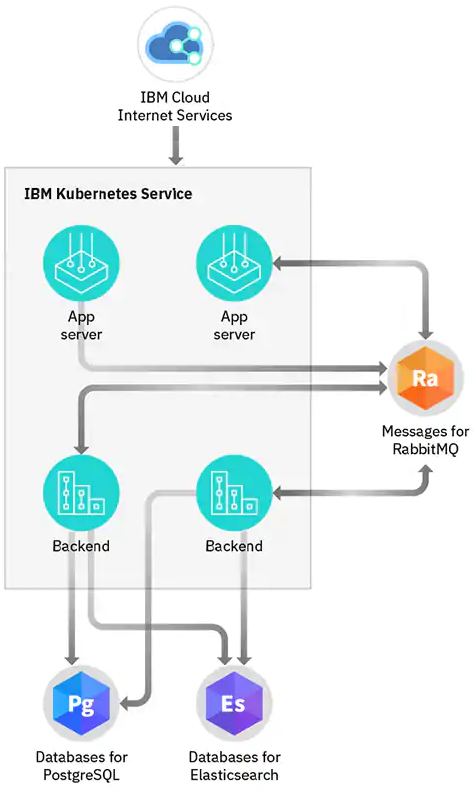
\includegraphics[width=0.7\textwidth]{/images/microservices/postgres.png}}
		\caption{Scalable SafeStreets architecture to handle millions of users.}
	\end{figure}
	\FloatBarrier
	\end{comment}
	\item \textbf{Statistics Database - \href{https://cloud.ibm.com/catalog/services/databases-for-postgresql}{Relational PostgreSQL Cloud Database}}: The Statistics Database where all the application usage statistics are. 
	These are not so important data so for what concerns the replication, it will not physically duplicated by us, but we rely on the internal data replication of IBM.
	\\As already stated, IBM Cloud Databases allows to scale disk and RAM to best fit the application requirements, but in this case is defined a maximum number of resources to be allocated because the statistics page is not a SafeStreets core functionality.
	After the deployment, everyone can query this database trough an apposite microservice, but the write access is restricted only to enabled services inside the IBM Cloud VPN.
	\item \textbf{Suggestion Database - \href{https://cloud.ibm.com/catalog/services/cloudant}{IBM Cloudant}}: This database represents the core heart of the memory that stores all the data that comes from the AI and Data Mining algorithms.
	\\Our system will be configured such as when it detects that is in a low-traffic moment, if it's in a time shift to be configured (late night) then it will start to mine the data of the past day to find possible suggestion to unsafe areas. When it finishes, the newly created suggestion will be stored in this database.
	\\As every suggestion comes from an Artificial Intelligence agents, it would be substantially different in structure from each other, and so it needs to be stored in a NoSQL database such as Cloudant. Figure \ref{fig:jsondoc} shows some possible documents that can be stored inside this database.
	\\This instance of Cloudant will be configured to accept read-only queries only from verified Public Police Officers.
	\begin{figure}[h!]
		\begin{lstlisting}
		{
		  "infraction": "Illegal parking",
		  "timeShift": 2019
		  "area": "Via Bassini",
		  "reportsCount": 1821,
		  "ticketsGiven": 1437,
		  "unsafeArea": true,
		  "incidents": 24,
		  "causedDeath": false,
		  "suggestions": [
			{
			  "suggestion": "Avoid illegal parking"
			  "actions":
			    [ 
				  {
				    "action": "Warn drivers with a flyer",
				    "score": 60.2
				  },
				  {
				    "action": "Make more tickets",
				    "score": 58.7
				  }
			    ]
			},
			{
			  "suggestion": "Make ZTL from 5PM"
			  "actions":
			    [ 
			      {
			        "action": "Install cameras",
			        "score": 80.2
			      }
			    ]
			}
		  ]
		}
		\end{lstlisting}
		\caption{Example of suggestion document.}
		\label{fig:jsondoc}
	\end{figure}
	\FloatBarrier
	
	
	%TODO: Add schema model
	\begin{comment}
	\begin{figure}[h!]
	\makebox[\textwidth]{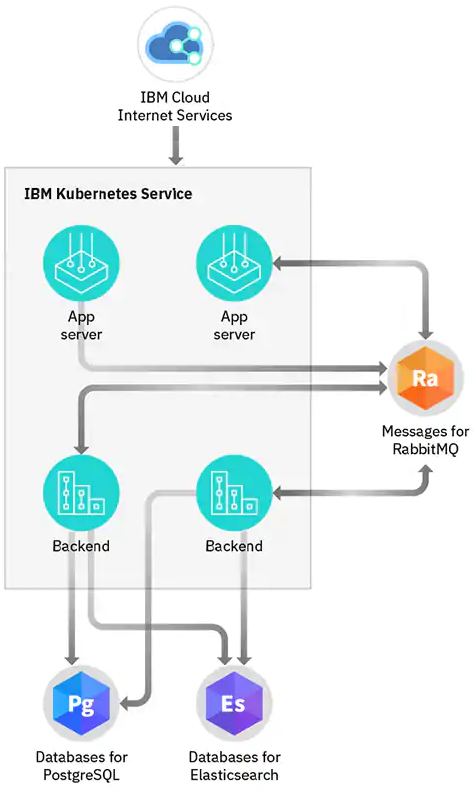
\includegraphics[width=0.7\textwidth]{/images/microservices/postgres.png}}
	\caption{Scalable SafeStreets architecture to handle millions of users.}
	\end{figure}
	\FloatBarrier
	\end{comment}
	
	%TODO: Add hash DB
	
	
\end{itemize}